\documentclass[11pt]{article}
\usepackage{amssymb}
\usepackage{algpseudocode}
\usepackage{algorithm}
\usepackage{setspace}
\usepackage{graphicx}
\graphicspath{ {./images/} }
\usepackage{hyperref}
\usepackage{siunitx}
\usepackage{amsmath}
\usepackage{caption}
\usepackage{subcaption}

\hypersetup{
    colorlinks=true,
    linkcolor=blue,
    filecolor=magenta,      
    urlcolor=cyan,
}

\title{MSc Project - Binding Affinity Prediction of Protein-Ligand Complex}
\author{
        Abdus Salam Khazi\\
        \href{mailto:abdus.khazi@students.uni-freiburg.de}
                {abdus.khazi@students.uni-freiburg.de}\\ \\
        \href{https://github.com/abduskhazi/MSc-Project}
                {Github Repository} \cite{github_repository} \\ \\
        Supervisors:
        \begin{tabular}{ll}
			Simon Bray \&
			Alireza Khanteymoori
		\end{tabular}
       }
	
\begin{document}

\maketitle
\date{}
\tableofcontents
\newpage

\section{Abstract}
\newpage

\section{Introduction}

\subsection{Biological Background}
Proteins are the workhorses of our body.  They are necessary for many important functions in the body.  Ligands are molecules that bind to proteins to form protein-ligand complexes.  They can be molecules that the protein transports (e.g., a Haemoglobin transporter) or act as stimulating agents.  In addition to this, they can also start/stop the protein from doing its function.  The correct functioning of these protein-ligand complexes is essential for any living organism.

The study of protein-ligand complexes is an intrinsic part of the drug discovery field.  It is because drugs are small molecules that act as ligands.  As the drug molecules (ligands) bind to the target proteins, they can artificially influence the protein behavior.  This binding between protein and ligand causes a therapeutic effect.

\begin{figure}[htb]
  \centering
    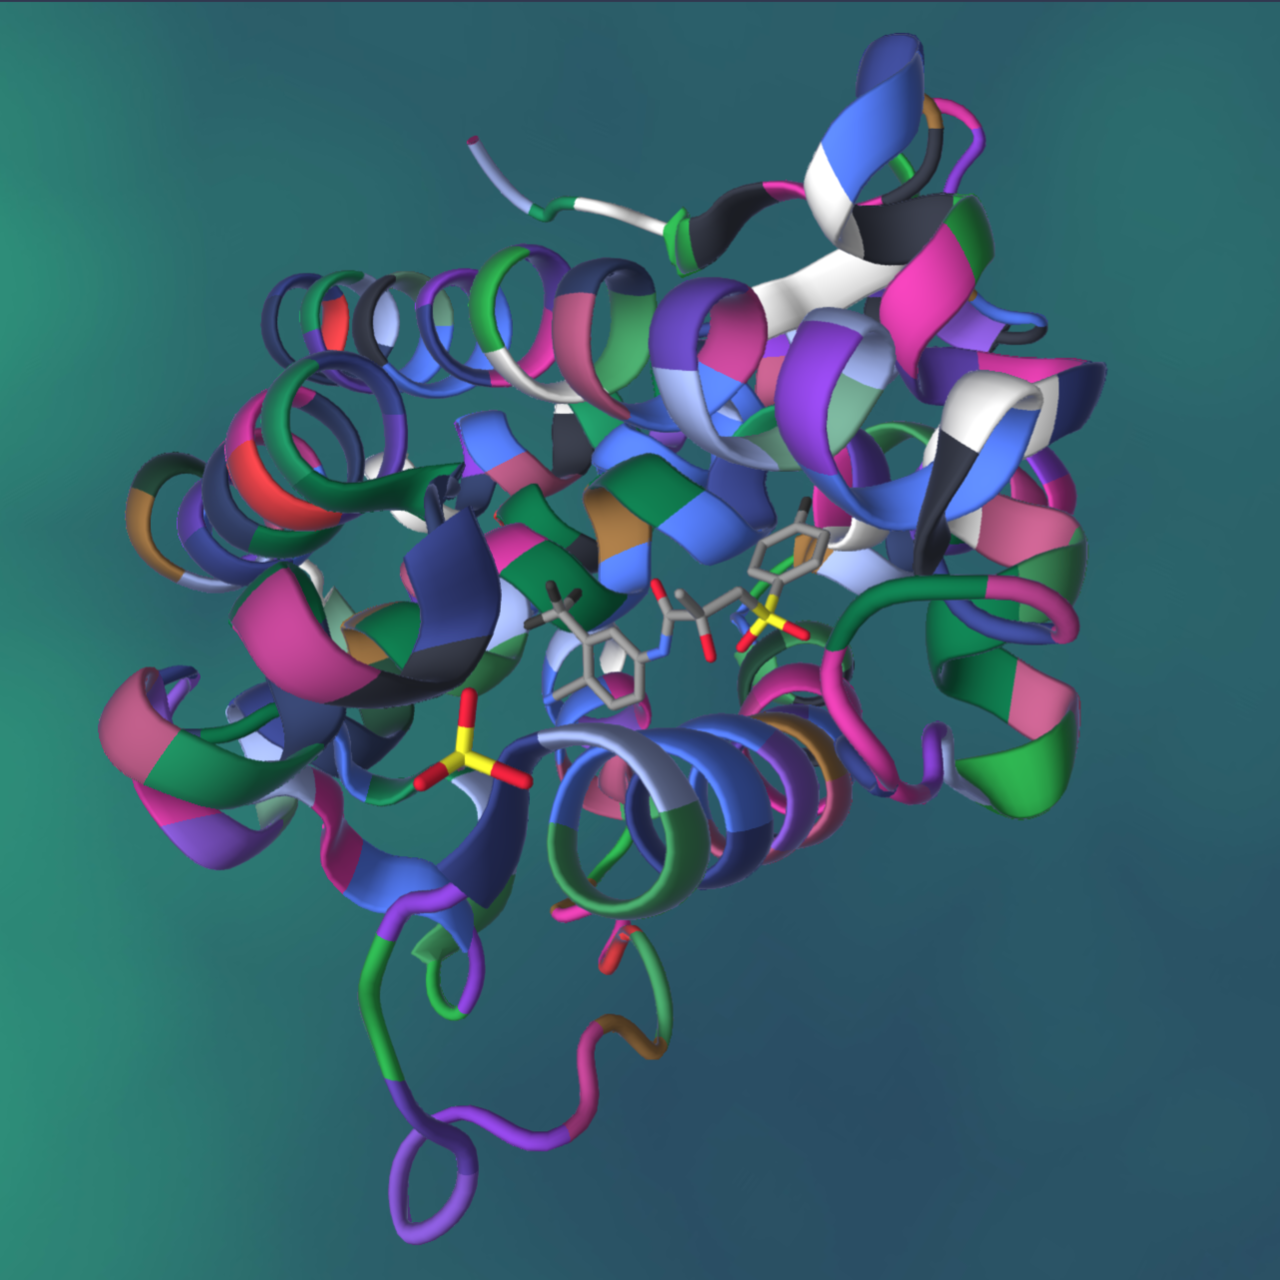
\includegraphics[scale=0.15]{images/pl_complex}
    \caption{Haemoglobin transporter protein.  \cite{PL_complex_introduction}}
    \label{fig:HaemoglobinTransporterImage}
\end{figure}


When a target drug candidate is found,  one has to answer questions like - How easily does the drug bind to the target protein? Does it bind to any other protein - If so, is it desirable? Does it have any unforeseen effect on the protein function? etc...  To answer these questions biologists and pharmacists conduct wet-lab experiments that are expensive.

One way to reduce the cost of these experiments is to make a data-driven selection of the drugs.  Using experimental data collected over many years, one can build models to predict the behavior of the proposed drug computationally.  These 'In-Silico' computational methods can aid in the elimination of undesirable drugs as well as guide the drug selection process.

This project aims to answer one of the above questions - How well does a given drug bind to the target protein? This is determined computationally by building a machine learning model that trains on the previous data.  Using this model,  the goal of the project is to reduce drug discovery costs. 

\subsection{Understanding Binding Affinity}
The binding affinity between a protein and a ligand is quantified by the $K_d$, $K_i$ and $IC_{50}$ measures in the PDBBind Data bank.
Here $K_d$ refers to disassociation constant, $K_i$ refers to the inhibition constant, and $IC_{50}$ refers to 
inhibitory concentration 50\%.
The reason for having different measurements is because it is not possible to use the same measurement techniques
for all biological complexes/processes.

To understand $K_d$, consider a protein and a ligand binding and unbinding continuously in a kinetic system.
In this system, let $[P]$, $[L]$, and $[PL]$ represent the concentrations of the Protein, the Ligand, and the Protein-Ligand complex respectively.
This is represented by the following equation:
$$[P] + [L] \rightleftharpoons [PL]$$
The binding affinity $K_d$ can be quantified by using the concentrations in the above system at equilibrium.
$$K_d = \frac{[P][L]}{[PL]} = \frac{k_{-1}}{k_1}$$
where $k_{-1}$ is the disassociation rate constant and $k_1$ is the association rate constant.
Similarly, $K_i$ and $IC_{50}$ are defined using concentration albeit non-trivially. 
\cite{binding_affinity_description}

\subsection{PDBBind Dataset}
Over the last few decades, researchers have been successful in building a single data archive for proteins.  This archive, called \textbf{Protein Data Bank} \cite{pdb_homepage}, holds 3-D structural data of the proteins determined by experiments like X-ray crystallographic, Nuclear magnetic resonance (NMR), and cryoelectron microscopy (cryoEM).  A subset of this data also contains information about how well a given protein and ligand bind together.  It is called binding affinity between a protein and ligands.  (It also contains data about protein-protein complexes that this project does not deal with)
\cite{pdbank_history}

As the protein-ligand binding affinity is studied here,  only the relevant data should be filtered out from \textbf{Protein Data Bank}.  This is already done by the maintainers of the \textbf{PDBBind Data Bank}.
\cite{pdbbind_introduction}
Using the curated protein-ligand affinity data present in the PDBBind Data bank,  a machine learning model that learns to predict the affinity is built.

\section{Problem Formulation}
\subsection{Problem Overview}
\label{ProblemOverviewlabel}
The problem that is solved is - \textit{Given $K_d$/$K_i$/$IC_{50}$ for various complexes in the PDBBind Data bank,
can this affinity measure be predicted for new protein-ligand complexes?}
Figure~\ref{fig:plproblemclassification} shows how the Protein-Ligand problem can be classified.

\begin{figure}[htb]
  \centering
    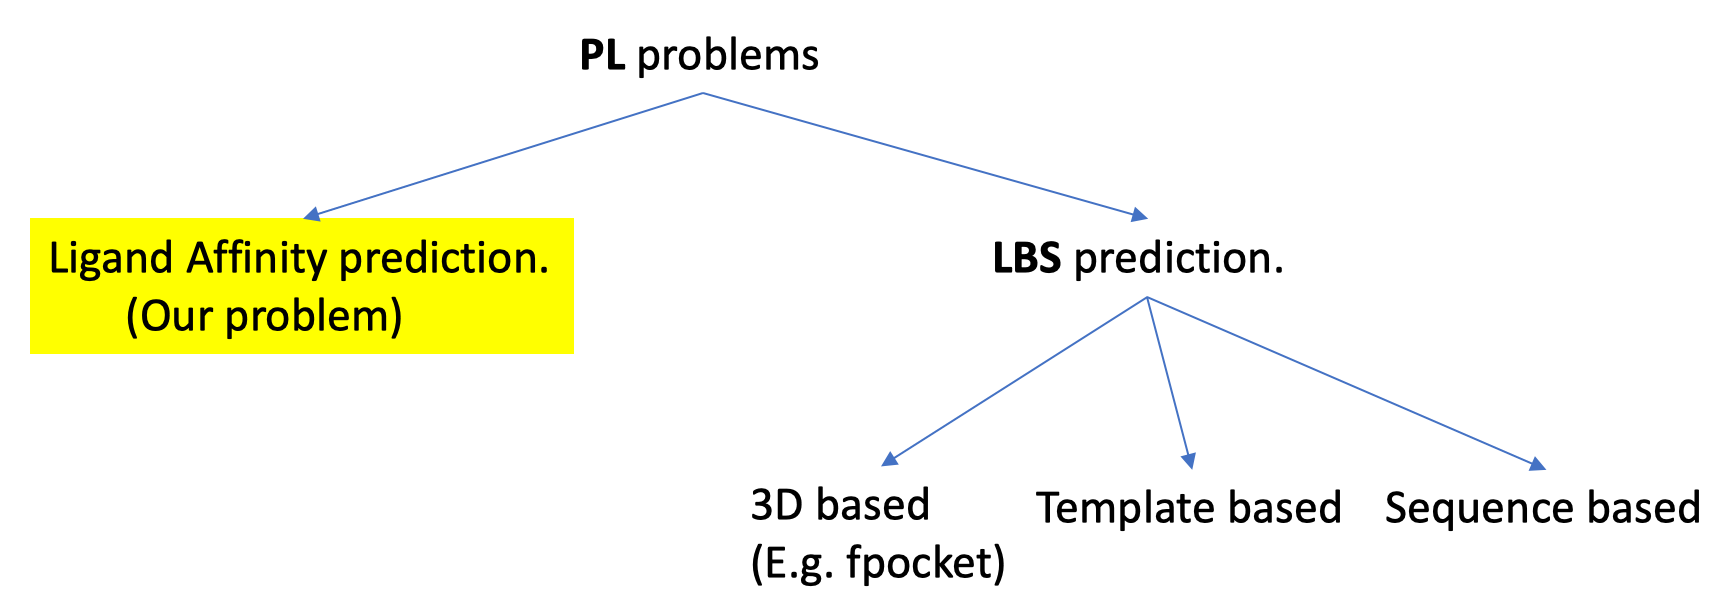
\includegraphics[scale=0.35]{images/pl_problem_classification}
    \caption{Protein-Ligand problem classifcation.}
    \label{fig:plproblemclassification}
\end{figure}

The binding of proteins and ligands is heavily influenced by their respective 3D structures.
Figure~\ref{fig:lockandkey} illustrates a hypothesis called \textit{Lock and Key}.
The shape of the protein's binding location and the shape of the ligand must be complementary for the binding.

\begin{figure}[htb]
  \centering
    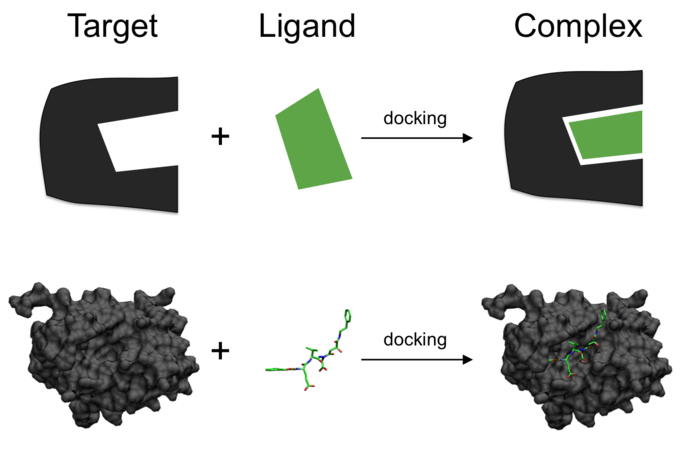
\includegraphics[scale=0.7]{images/lock_and_key}
    \caption{Lock and Key hypothesis in molecular docking.  \cite{lockandkeyformatpng}}
    \label{fig:lockandkey}
\end{figure}

The other parts of the protein are not involved in the binding process directly.
Hence,  only the features of the binding location were obtained.
Any potential binding location in the 3D structure of a protein is called a pocket.
A 3D-based LBS prediction package called \textit{fpocket} was used to find the potential pockets.
A submodule in the package called \textit{dpocket} is used to extract the binding pocket's features.

To give a plug-and-play input to the model,  the features of proteins and ligands were kept distinct till the training phase.
That is,  the combined features were not used in any pre-processing of the ML pipeline e.g. feature reduction.
This helps the model to provide the binding affinity between any protein and any ligand.



\subsection{Overview of file formats}
The \textbf{PDBBind Data bank} extracts information about the PL complexes from the \textbf{Protein Data bank} and creates the following files for every complex
\begin{itemize}
\item \textbf{PDB Format} - For the Protein.
\item  \textbf{Mol2} - For the ligand.
\item \textbf{SDF} - For the ligand.
\end{itemize}

All of the above formats contain the 3D information that is essential in the prediction of the binding affinity.
All the above-mentioned formats use the \textbf{XYZ format} internally to represent the 3D structure of their molecules.

\subsubsection{XYZ format}
\label{xyz_format}
XYZ format is a chemical file format that represents the geometry of a molecule.
It specifies the number of atoms and their Cartesian X, Y, Z coordinates hence the name XYZ format.
The following text illustrates the XYZ format.
Section \ref{XYZFileexampleref} gives an example.
\cite{XYZ_format}
\begin{verbatim}
<number of atoms>
comment line
<element> <X> <Y> <Z>
...
\end{verbatim}

The unit of distance used is Angstrom (\si{\angstrom}).  \SI{1}{\angstrom} $ = 10^{-10}$ m.
\cite{XYZ_format}

\subsubsection{PDB format}
PDB format is a human-readable file format used to represent the protein molecules (macromolecules).
Within the PDB format,  the coordinates of atoms are represented like the XYZ format [see \ref{xyz_format}].
Because of the 3D information in this format,  molecular visualization of proteins is possible with specialized software. 
It also contains information about atomic connectivity and the protein's primary,  secondary,  tertiary,  and quaternary structures.
\cite{pdb_file_format}
\cite{understanding_pdb_format}
Please see \cite{examplePDBFile} for an example pdb file.


\subsubsection{Structure Data File (SDF) Format}
SDF format file is a Chemical Table file (CT File) that contains a structure of the molecule in the X, Y, Z format.
It contains information like atomic bonds,  connectivity information,  molecular weight,  and molecular formula. \cite{SDFformat}
Section \ref{SDFFileexampleref} illustrates the SDF file format.

\subsubsection{Mol2 format}
Similar to the SDF format,  Mol2 also represents the 3D structure of a molecule in the X, Y, Z format.
It contains the atomic bond and connectivity information but does not contain the other data like molecular weight and formula.
The ligands given in this format were used because more ligands in mol2 format could be processed with the RDKit feature extractor.
Section \ref{MOL2Fileexampleref} illustrates the Mol2 file format.

\subsubsection{SMILES format}
SMILES is an acronym for Simplified Molecular-Input Line-Entry System.
It represents a molecule using an ASCII string.
Using the 3D data in SDF and Mol2 formats,  an atomic graph representation could be created.
Using this graph the SMILES string for the molecule can be generated.
The SMILES format itself is not very helpful for us as one would lose the 3D structural information after converting to it.
\cite{smilesformat}

\subsection{Extraction of features}
As the file formats are different for proteins and ligands,  different tools were used to extract their features.
\subsubsection{Ligand Features using RDKit}
RDKit is an open-source cheminformatics software \cite{rdkitofficalpage}.
The core data structures and algorithms of RDKit are written in C++ and the
python wrappers are generated using Boost.Python.
Using the module, \textit{RDKit.Chem.Descriptors} $402$ features were extracted for each ligand \cite{rdkitbioinformaticsfreiburg}.
Each descriptor value is taken as a real number,  hence the input space of ligand features is $\mathbf{R}^{402}$ before any feature elimination.

\subsubsection{Protein Features using fpocket/dpocket descriptors}
\textit{Fpocket} stands for "Find pocket" whereas \textit{Dpocket} stands for "Describe pocket".
\textit{Fpocket} uses 3D Voronoi tessalation and the concepts of "Alpha Spheres" to find out pockets in the protein structure \cite{fpocketmanual} \cite{voronoitesselationshortvideo}.
Given a protein PDB file,  the descriptors of all pockets in the protein could be extracted.
For every pocket,  55 descriptors were obtained in total. They were taken as real values, $\mathbf{R}$.
Hence the input space for protein features is $\mathbf{R}^{55}$.


To get the descriptors of the ligand-binding pockets,  \textit{Dpocket} was used.
\textit{Dpocket} is provided with the protein PDB file and the ligand ID of the PL complex as input.
It generates 3 files as output files,  namely,  dpout\_fpocketp.txt, dpout\_fpocketnp.txt,  and  dpout\_explicitp.txt.
\begin{itemize}
\item \textbf{dpout\_fpocketp.txt}.
This file contains the descriptors (a.k.a features) of all pockets that are considered to be binding pockets based on a binding criterion.
The ligand can bind at different locations (pockets) in the protein 3D structure.
Hence,  there may be features of more than 1 pocket in this file.
\item \textbf{dpout\_fpocketnp.txt}.  This file contains the descriptors of all pockets that are non-binding according to the criteria.
\item \textbf{dpout\_explicitp.txt}.  An explicit pocket is defined as a pocket consisting of all vertices/atoms situated at a specific distance from the ligand in the PL complex.
This distance is 4 \r{A} by default.
This file contains the descriptors of all explicit pockets in the PL complex. 
\end{itemize}

In the project,  dpout\_fpocketnp.txt files were not used as they contain the non-binding pockets.
In the other 2 files,  the pocket descriptors that were given by dpout\_fpocketp.txt were preferred as explicitly defined pockets are heavily biased towards the ligand.

\section{Feature selection}
\subsection{Requirement of feature selection}
Both the protein and the ligand are equally responsible for the affinity of the PL complex.
Hence their descriptors were concatenated to get a high dimensional $\mathbf{R}^{457}$ input for the model.
There are a couple of issues with using all of the descriptors.
\begin{itemize}
\item The amount of data is not very large. 
For example,  only $\approx$ 35000 data points could be obtained after concatenating the ligand features with the \textit{fpocketp} pocket descriptors.
\item The number of ligand descriptors $>>$ protein descriptors.
This creates a data imbalance and may lead the model to select only ligand features for their prediction.
\end{itemize}
Hence some methods to reduce the input dimensions are required.

\subsection{Feature Family analysis}
\label{CorrelationAnalysis}
All the features extracted from the PDB and the ligand files can be classified into various families.
Some of the important ones are - AUTOCORR2d\_, Chi, EState\_VSA,  PEOE\_VSA,  SMR\_VSA,  SlogP\_VSA,  VSA\_EState, and fr\_.
Figure~\ref{fig:correlationheatmap} shows the correlation matrix of 2 of the most interesting families AUTOCORR2d\_ and Chi.
As can be seen in the heatmap there is a heavy correlation within the families.
Hence a strategy to deal with this is also required.
The correlation heat maps for the other families are illustrated in Section \ref{CorrHeatMapsAppendix}.

\begin{figure}[htb]
    \begin{subfigure}[b]{0.45\textwidth}
         \centering
         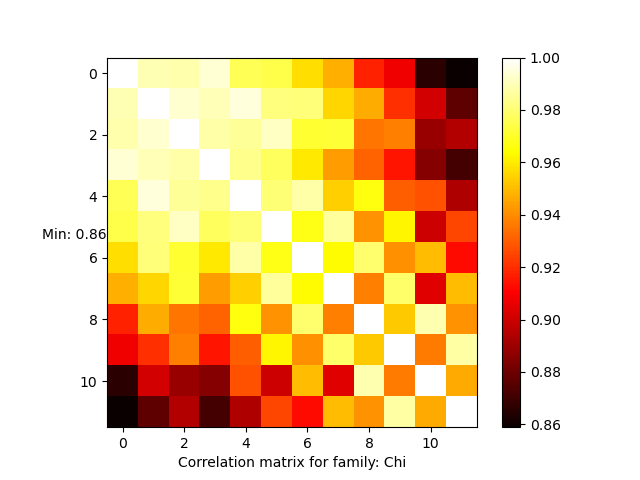
\includegraphics[scale=0.45]{images/correlationChi}
        \label{fig:correlationChi}
     \end{subfigure}
     \hfill
    \begin{subfigure}[b]{0.45\textwidth}
         \centering
         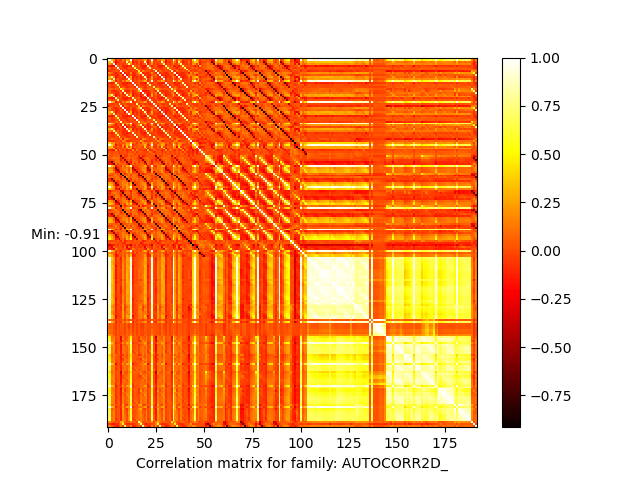
\includegraphics[scale=0.45]{images/correlationAUTOCORR2D}
        \label{fig:correlationfr}
     \end{subfigure}
     \caption{Correlation Heat Map}
     \label{fig:correlationheatmap}
\end{figure}

\subsection{Feature Selection Strategies}

%The data if it is complementary is better for solving the problem.
%The accuracy measure of the protein LBS prediction is the same as the dichotomous problems in math.

The features of proteins and ligands were selected separately.
This helps us make the model plug-and-play as discussed in section \ref{ProblemOverviewlabel}.
The best combination,  i.e Global Optima,  cannot be obtained practically by brute force algorithms.
This is because one would have to try $\binom{402}{k_1} * \binom{55}{k_1}$ ($k_1, k_2 \in \mathbf{I}^+$) possibilities which is impractical.
In the next subsections, a few feature selection strategies that were considered in this project are discussed.

\subsubsection{Selection by output correlation}
The \textit{pearson} and \textit{spearman} correlations of each feature were calculated against the output variable.
It was assumed that the features were either linearly related to the output (in the case of Pearson correlation) or had a monotonic relationship (in the case of Spearman correlation).
20 from the ligand descriptors that were most correlated to the output were selected as inputs to the model.  Similar 20 best features from the protein descriptors were selected.

\subsubsection{Using genetic algorithms}
Since the feature space is a non-continuous problem of combinatorial complexity,
genetic feature selection algorithms \cite{genetic_algorithm} were also studied.
Each feature was represented by a binary number, 1 for the inclusion of the feature and 0 for its exclusion.
Let $\mathbb{B}$ be a binary number $\{0,  1\}$.
Each feature selection $p \in \mathbb{B}^{456}$ (401 for ligands + 55 for proteins) is called a chromosome.
A "population" of $n$ chromosomes is maintained.
For each generation,  the best pairs of chromosomes are selected as parents.
The next generation is created by crossover and mutation of the chromosomes.
Algorithm~\ref{alg:GeneticAlgo} below gives complete pseudocode for this.

The scoring function used to select the best chromosome can vary according to the model type. [See Section~\ref{MachineLearningModelslabel}]

\begin{algorithm}
\caption{Selection of features for the model using genetic algorithm \cite{genetic_algorithm}}
\label{alg:GeneticAlgo}
\begin{algorithmic}[1]
\Procedure{GENETIC\_ALGORITHM\_BASED\_SELECTOR}{}
\State scoringfunction $\gets$ Get model specific scoring function
\State $ population = \{C_1, C_2, C_3... C_n\}$ $\in$ $\mathbb{B}^{456}$ (initial chromosomes).
\State best $\gets C_1$  \textit{// Arbitrarily initialized}
\State $i \gets 0$
\State $gen \gets$ number of generations to run.
      \For{\texttt{$i < gen$ with step 1}}
          \State $\{S_1, S_2, S_3... S_n\} \gets$ scoringfunction($population$) $\forall S_i \in \mathbf{R}$.
          \State \textit{// Do a tournament selection for the best chromosomes}
          \State $genetically\_better\_population \gets$ empty list
          \For{\texttt{$j < len(population)$}}
              \State Set $\gets$ random\_k\_selections($population$)
              \State $c \gets best($Set$)$ \textit{// Based on scoringfunction.}
              \State $genetically\_better\_population.add(c)$
          \EndFor
          \State $children \gets$ empty list
          \For{\texttt{$j < len(population)$ with step 2}}
              \State $P_1, P_2$ $\gets$ $population[j], population[j+1]$
              \State $c_1, c_2 \gets crossover(P_1, P_2)$
              \State $c_1 \gets mutation(c_1)$
              \State $c_2 \gets mutation(c_2)$
              \State $children.add(c_1, c_2)$
          \EndFor
          \State $population \gets children$
      \EndFor
\State return best($population$)
\EndProcedure
\end{algorithmic}
\end{algorithm}

\subsubsection{Manual Feature selection}
A selected list of 121 ligand descriptors was given by Simon Bray. 
All protein descriptors were used as they were only a few in number.

\section{Testing}
\subsection{Reproducibility}
Reproducible ML models are very crucial for verifying any project or research results. Due to the stochastic nature of many ML training processes, reproducing the exact model (and consequently the exact output) is a challenge. Two methods can be employed to produce verifiable results:
\begin{itemize}
\item Training many models and reporting the average results.
\item Controlling the randomness of the trained models. It is done by setting the seed of the pseudo-random algorithms.
\end{itemize}

The second approach was used in this project. Every script, when executed, reports an execution ID. This is the random seed used during the execution.  The exact results can be reproduced by using this execution ID as the first argument to the script.

\subsection{Model Quality Analysis}
The following function is predicted by the model
$$ \textrm{Binding affinity prediction} : \mathbf{R}^n \mapsto \mathbf{R} \;\; \textrm{where} \;\; n \in \mathbf{I}^+$$
Since the input space is multi-dimensional,  one cannot fully visualize the model as a function of the input space.
To get around this,
\begin{itemize}
\item \textit{Coefficient of determination} is reported. $R^2  \in (- \infty, 1.0]$ where $1.0$ is the best score. \cite{r_squared_score}
$$R^2(y, \hat{y}) = 1 - \frac{\sum_{i=1}^{n} (y_i - \hat{y}_i)^2}{\sum_{i=1}^{n} (y_i - \bar{y})^2} \;\; \textrm{where} \;\; \bar{y} = \frac{1}{n} \sum_{i=1}^{n} y_i \;\;
\textrm{and} \;\; \sum_{i=1}^{n} (y_i - \hat{y}_i)^2 = \sum_{i=1}^{n} \epsilon_i^2$$

\item A 2D scatter plot of expected values vs the model's output is plotted. 
\end{itemize}

A perfect model would have all the points on the $y = x$ line.  This corresponds to a $R^2$ score of $1.0$. 
Figure~\ref{fig:modelQualityVisualization},  shows the validation accuracy of a sample \textit{Random Forest Regressor} model.
$y\_validate$ ($x$ axis) represents the actual validation data.
$y\_validate\_pred$ ($y$ axis) represents the predicted output from the model.

\begin{figure}[htb]
  \centering
    \includegraphics[width=1.0\textwidth]{images/accuracy_validate}
    \caption{(Sample) Visualizing accuracy.  $R^2 \approx 0.805$.}
    \label{fig:modelQualityVisualization}
\end{figure}

%\includegraphics[scale=0.7]{accuracy_validate}
%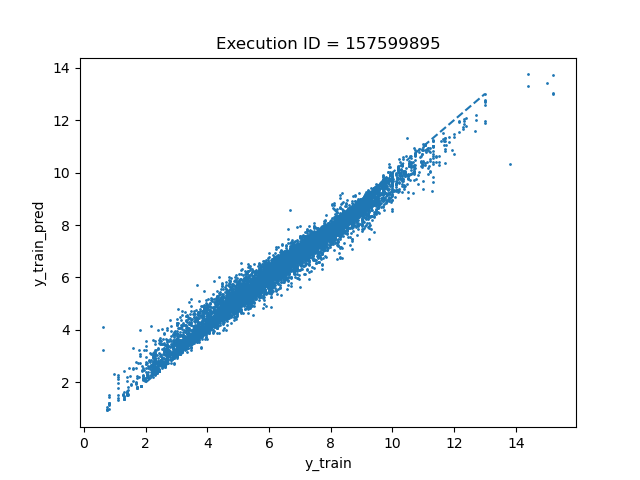
\includegraphics[scale=0.7]{accuracy_train}

\section{Machine Learning Models}
\label{MachineLearningModelslabel}
The following machine learning models were used:
\begin{itemize}
\item Linear Regression
\item Support Vector Regression
\item Rotation Forest Regression
\item Random Forest Regression
\end{itemize}

By far, the most impressive performance was given by Random Forest Regression.
Hence more time was spent on the Random Forest regression models to understand the reasons for their good performance.

Because of the lack of data, Deep Neural Networks were not suitable for this project. 
For example, if all the features were used to train a simple DNN model of size $[457,  20, 10,  1]$,  there would be 9350 parameters to train.  As only 16,000 data points were present to train the model,  the deep learning model would over-fit drastically.


\subsection{Data Preprocessing}
Before fitting the model,  a preliminary analysis of the data was performed.  This was necessary to train the models more reliably.

\subsubsection{Data cleaning}
Using principal component analysis (PCA) each feature's contribution in the variation of the data was analyzed. 
During this analysis, 2 issues were found:
\begin{itemize}
\item There was a ligand feature named IPC which had extremely small and extremely huge values e.g $k * 10^{39}$ where $k \in (0,1]$.
Hence we scaled this feature using a logarithm function.
This was done for numerical safety during the training of our models.
The effect of this scaling on the cumulative PCA is shown in Figure~\ref{fig:PCAAnalysis}.

\begin{figure}
     \centering
     \begin{subfigure}[b]{0.45\textwidth}
         \centering
    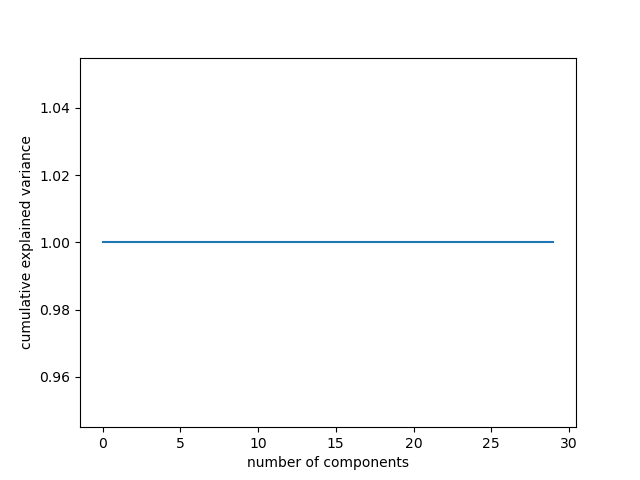
\includegraphics[scale=0.5]{images/pcaligandanalysisIPC}
    \caption{With original Ligand feature IPC}
    \label{fig:pcaproteinanalysisIPC}
     \end{subfigure}
     \hfill
     \begin{subfigure}[b]{0.45\textwidth}
         \centering
        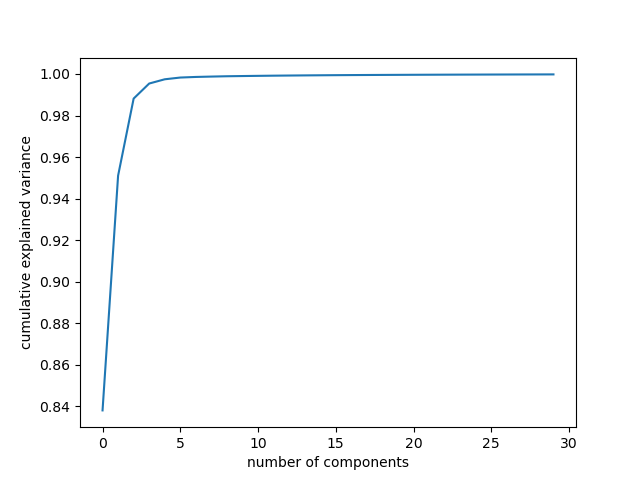
\includegraphics[scale=0.5]{images/pcawithscaledIPC}
        \caption{With log scaled Ligand feature IPC}
        \label{fig:pcawithscaledIPC}
     \end{subfigure}
     \caption{Cumulative PCA of ligand features}
     \label{fig:PCAAnalysis}
\end{figure}

\item There were a lot of NaN (Not a number) and zeros in our data.  Perhaps these descriptors did not make sense for some of the ligands. While the presence of 0s was harmless,  we made sure that we removed all NaN values before we input the data into our model.  Figure~\ref{fig:pcaproteinanalysis} shows cumulative PCA of the protein features. 
\end{itemize}

\begin{figure}[htb]
  \centering
    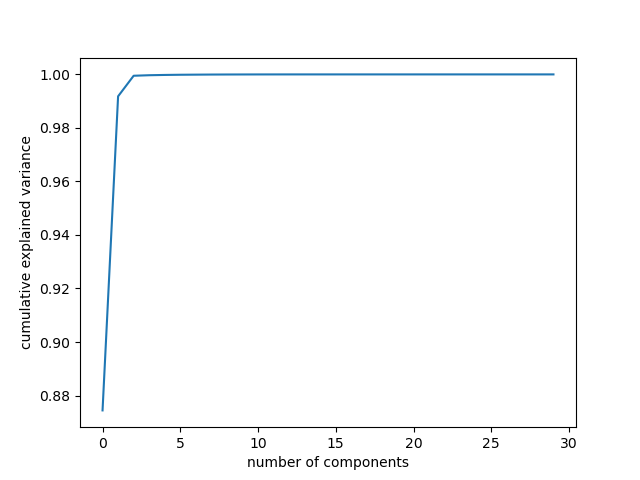
\includegraphics[scale=0.7]{images/pcaproteinanalysis}
    \caption{cumulative PCA of protein features}
    \label{fig:pcaproteinanalysis}
\end{figure}

It must be noted that the scaling of ligand feature IPC must be done before we use the model for the prediction of new data.
This is a limitation of our model.

\subsubsection{Dealing with measurement resolution}
Atomic structures produced using X-ray crystallography always have a particular resolution associated with them (\si{\angstrom} units). The structural detail of the 3D image is inversely proportional to the resolution.
As shown in a small excerpt of the PDB Databank INDEX file,  we have a resolution measurement for each of the complexes (or data points).

\begin{verbatim}
# ==============================================================================
# List of protein-ligand complexes with known binding data in PDBbind v.2019
# 17679 protein-ligand complexes in total, sorted by binding data
# Latest update: Dec 2019
# PDB code, resolution, release year, -log Kd/Ki, Kd/Ki, reference, ligand name
# ==============================================================================
3zzf  2.20  2012   0.40  Ki=400mM      // 3zzf.pdf (NLG)
3gww  2.46  2009   0.45  IC50=355mM    // 3gwu.pdf (SFX)
1w8l  1.80  2004   0.49  Ki=320mM      // 1w8l.pdf (1P3)
\end{verbatim}

Using the resolution, we devised the following 2 ways to calculate the weight of each data point.
\begin{itemize}
\item Hyperbolic formula: $  W_i = \frac{ \mathrm{\max{R_{1 ...  n}}}}{R_i}  $
\item Linear formula: $ W_i = (\mathrm{\max{R_{1 ...  n}}} + 1) - R_i $
\end{itemize}

Where $R_i$ is a resolution of a given data point.
We found that $\mathrm{\max{R_{1 ...  n}}} \approx 5$ \si{\angstrom} in our data.
It is necessary to add 1 to the max resolution in the linear formula to avoid data points with 0 weight.
The formulae are depicted in Figure~\ref{fig:graphingformula}.
Figure~\ref{fig:resolutiondistribution} shows the distribution of data points as a function of resolution.
The resolution of the measurements ranges from 1 \si{\angstrom} to 5 \si{\angstrom} approximately.

\begin{figure}
     \centering
     \begin{subfigure}[b]{0.45\textwidth}
         \centering
    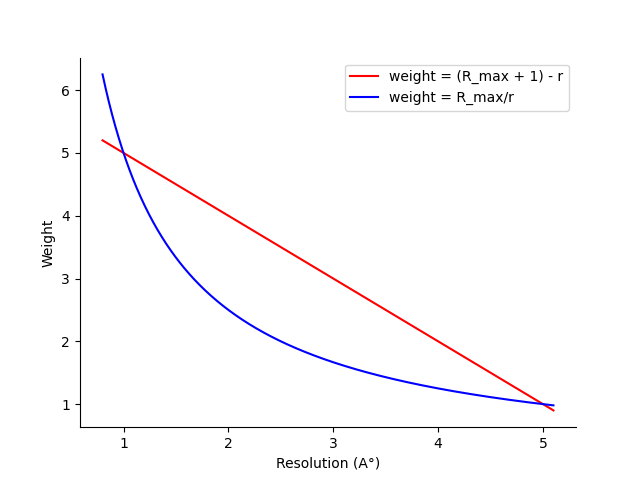
\includegraphics[scale=0.5]{images/graphingformula}
    \caption{Weight calculation formulae}
    \label{fig:graphingformula}
     \end{subfigure}
     \hfill
     \begin{subfigure}[b]{0.45\textwidth}
         \centering
        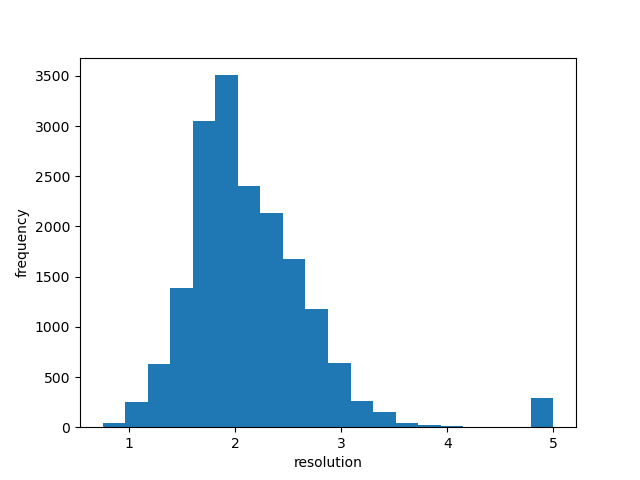
\includegraphics[scale=0.5]{images/resolutiondistribution}
        \caption{Resolution distribution}
        \label{fig:resolutiondistribution}
     \end{subfigure}
     \caption{ Weight calculation and resolution distribution}
     \label{fig:ResolutionWeightStats}
\end{figure}

Figure~\ref{fig:WeightDistribution} shows the distribution of the weights obtained from our data for the linear and hyperbolic case.
In Figure~\ref{fig:linearweightdistribution},  we see that linear weighting gives data points with a higher weight as compared to hyperbolic weighting.
This makes intuitive sense because as shown Figure~\ref{fig:resolutiondistribution}, 
most of the data points have a resolution around 2 \si{\angstrom}.
Since linear weighting around 2 \si{\angstrom} is higher, the linearly weighted data points will have a higher weight on average.

\begin{figure}
     \centering
     \begin{subfigure}[b]{0.45\textwidth}
         \centering
    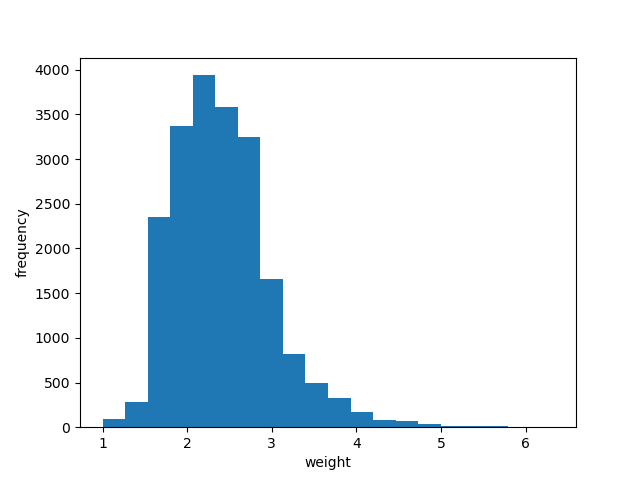
\includegraphics[scale=0.5]{images/hyperbolicweightdistribution}
    \caption{Hyperbolic weighting}
    \label{fig:hyperbolicweightdistribution}
     \end{subfigure}
     \hfill
     \begin{subfigure}[b]{0.45\textwidth}
         \centering
        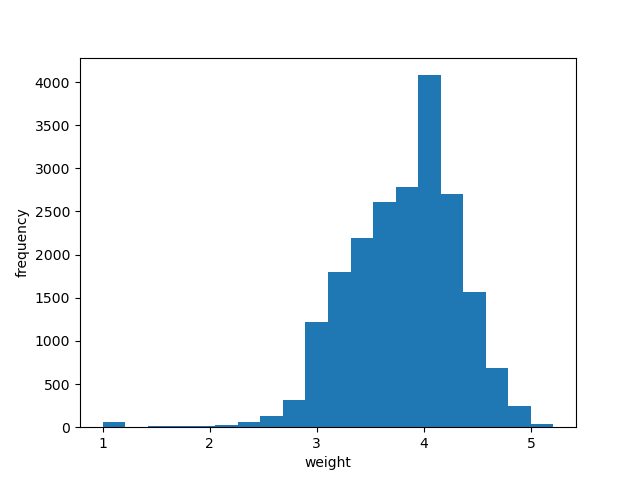
\includegraphics[scale=0.5]{images/linearweightdistribution}
        \caption{Linear weighting}
        \label{fig:linearweightdistribution}
     \end{subfigure}
     \caption{Weighting of our data points (Excluding the test set)}
     \label{fig:WeightDistribution}
\end{figure}

We employed 2 strategies to use the calculated weights in our models.

\begin{itemize}
\item Duplicating the data points.
\item Using the weights directly in the fit function.
\end{itemize}

After the duplication, we get $\approx$39,000 data points for the linear weighting formula and training and  $\approx$62,000 for the hyperbolic weighting.

\subsection{Linear regression}
Linear regression fits a linear model to a given data.
It tries to minimize the square of errors between the predicted output value and the actual output value.
This is the cheapest model (computationally) that we used to fit our data.
Table~\ref{table:1} shows the overview of our analysis with this model.
Figure~\ref{fig:BestLinearModel} shows the best results obtained with linear regression.

\begin{table} [h!]
\centering
\resizebox{\linewidth}{!} {
\begin{tabular}{ | c | c | c | c | c | c | }
\hline
\textbf{No.  features} & \textbf{Feature selection} & \textbf{Weighting} & \textbf{Training} & \textbf{Validation} & \textbf{Testing} \\ [0.5 ex]
\hline \hline
457 & - & - & 0.456 & 0.433 & 0.412\\
\textbf{457} &  \textbf{-} & \textbf{Hyperbolic} & \textbf{0.452} & \textbf{0.431} & \textbf{0.420}\\
457 & - & Hyperbolic duplication & 0.465 & 0.424 & 0.419\\
457 & - & Linear & 0.455 & 0.430 & 0.416\\
457 & - & Linear Duplication & 0.460 & 0.428 & 0.407\\
49 & Genetic\footnotemark[1] & Hyperbolic & $\approx$0.373 & $\approx$0.393  & $\approx$0.402\\
40 & Pearson Correlation & Hyperbolic & 0.288 & 0.276  & 0.286 \\ 
40 & Spearman Correlation & Hyperbolic & 0.291 & 0.280  & 0.289 \\ 
176 & Manual & Hyperbolic & 0.364  & 0.342  & 0.389\\ [1ex]
\hline
\end{tabular}
}
\caption{$R^2$ scores of the Linear Regression Model}
\label {table:1}
\end{table}

\footnotetext[1]{Approximately reproducible as the reproducibility module was introduced later.}

\begin{figure}
     \centering
     \begin{subfigure}[b]{0.45\textwidth}
         \centering
         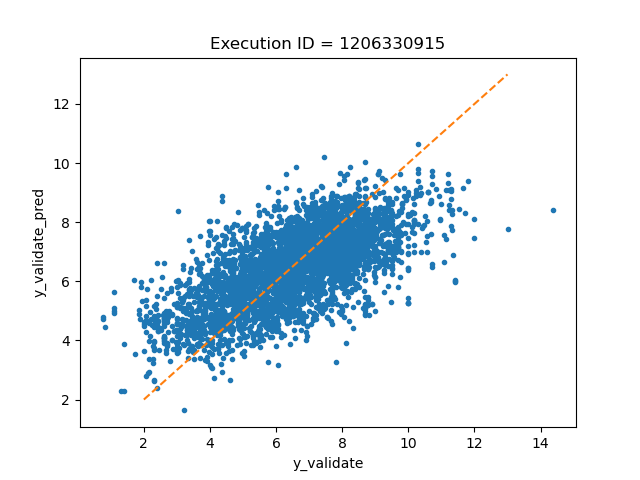
\includegraphics[scale=0.45]{images/accuracyValidateLGHyperbolic}
         \caption{Validation Accuracy}
        \label{fig:accuracyValidateLGHyperbolic}
     \end{subfigure}
     \hfill
     \begin{subfigure}[b]{0.45\textwidth}
         \centering
         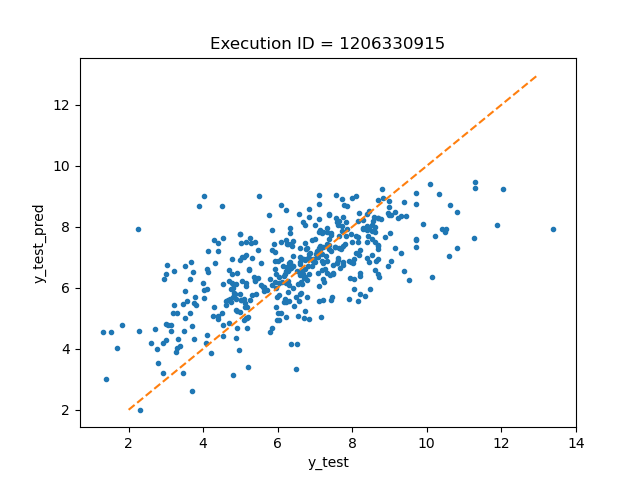
\includegraphics[scale=0.45]{images/accuracytestLGHyperbolic}
        \caption{Test Accuracy}
        \label{fig:accuracytestLGHyperbolic}
     \end{subfigure}
     \caption{Linear Model using Hyperbolic weighting and all 457 features.}
     \label{fig:BestLinearModel}
\end{figure}

The reason for the low $R^2$ score is that linear models assume strong linearity between the input variables and the output variable.
This is not always true.
One anomaly in the results is that there are some cases where the validation and testing results seem to be better than the training result.
However, this is not always the case. 
The results highly depend on the seed.
If the seed changes,  the train/test data split gives different data for training and different data for validation.
What is important for the validity of our model is that the results remain in a reasonable range.

In the linear regression model,  we used genetic algorithms to reduce both the large feature space and to eliminate correlated features within the families. 

\subsubsection{Score function of genetic feature selection}
\label{GenerationScoringFunction}
Since the fitting of the linear regression model was very cheap, we could afford to refit the model every time in our genetic algorithm.
We had 2 objectives at hand
\begin{itemize}
\item Get the best performing model.
\item Reduce the number of input features to make our model simple and explainable.
\end{itemize}
The above objectives are not always against each other.
This is because removing a feature that has no correlation (or random correlation) with the output may improve the model whereas removing a feature that the output is highly correlated on degrades the model.

Hence,  taking inspiration from the hypervolume-based multi-objective optimization, we designed the following score function.
$$
\textrm{score} = \mathbf{R}^2 \textrm{score} * \textrm{Features Eliminated}
$$
Figure~\ref{fig:scorefunctionfigure} provides a graphical depiction of the score function.
Here the score function represents the area of the square formed between a given point and the origin.
Trying to improve the score means,  it will try to eliminate more features as well as try to get a higher $R^2$ score.
In the example below,  the point $a$ is preferred over $b$ as it gives almost the same $R^2$ score and eliminates a larger number of features.
Another advantage of this score function is that we do not need to keep the values of both components (i.e. \textit{features eliminated} and \textit{$R^2$} score) in a similar range.
Hence we need not worry about scaling any of these components.

\begin{figure}[htb]
  \centering
    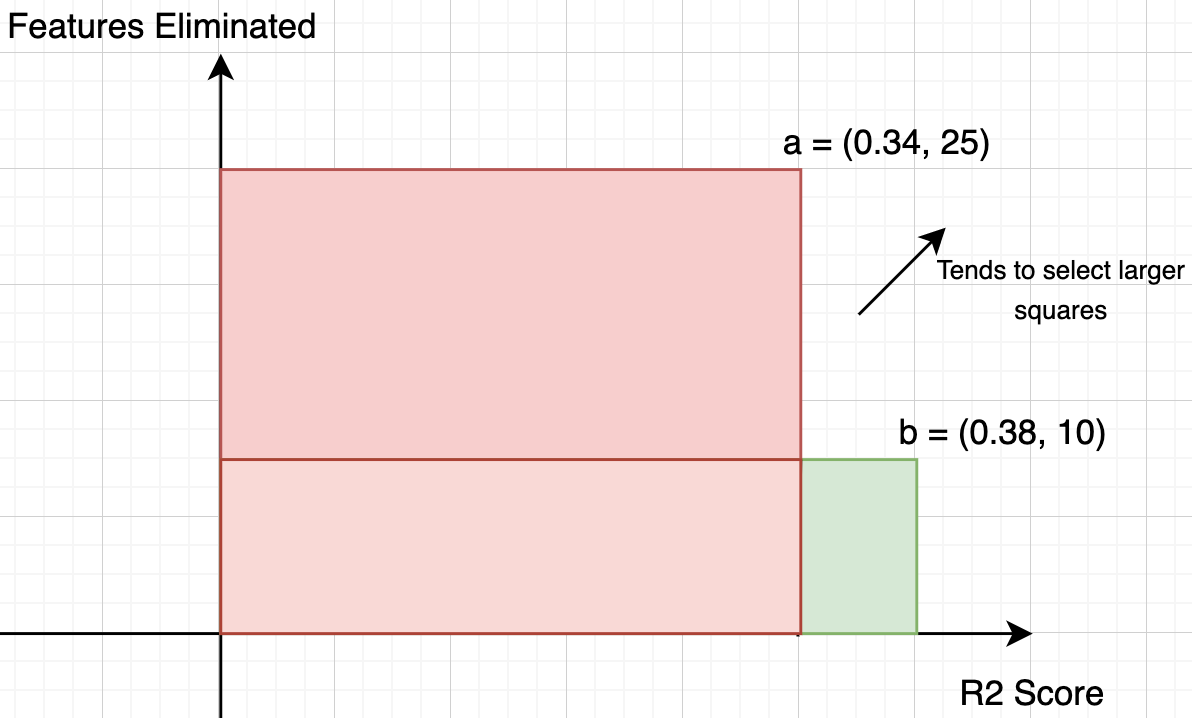
\includegraphics[scale=0.5]{images/scoreFuntionMultiObject}
    \caption{Genetic Algorithm score function representation.}
    \label{fig:scorefunctionfigure}
\end{figure}

\subsubsection{Initialization strategies of population}
Two main strategies were used to initialize the population for the genetic algorithm:
\begin{itemize}
\item \textbf{Random Initialization}.  A population of $2400$ chromosomes was randomly initialized and run for $500$ generations.
\item \textbf{Specific Initialization}.  Here,  the initial population was kept at $457$.
The algorithm was run for $2000$ generations.
Each chromosome in the population had 1 distinct feature excluded.  The following represents the initialization of the chromosomes.

$
c_1 = [0 1 1 1 1 ......  1 1]
$ \\
$
c_2 = [1 0 1 1 1 ......  1 1]
$ \\
$
c_3 = [1 1 0 1 1 ......  1 1]
$ \\
$
... 
$ \\
$
c_{457} = [1 1 1 1 1 ......  1 0]
$

The rationale was that using the above score function we could go to a local minimum by eliminating the worst performing features rather than trying to select the best performing features as in the case of random initialization.
\end{itemize}

Both the initialization strategies gave similar results as shown in Table~\ref{table:1}.

\subsection{Random Forest Regression}
\label{RandomForestRegressionLabel}
Random forest regression is an ensemble ML model of regression trees.
When training each tree,  the algorithm finds out which feature value can divide the data into 2 groups to yield the lowest sum of squared values on both sides (The criterion can be different as well e.g. lowest absolute error).
Then each of the sub-data is split recursively till a stopping criterion (e.g. a set number of data points in the leaf).

For each tree,  a subset of the data is used for training. 
The subset of data is sampled with replacement a.k.a bagging.
After training,  the bunch of "Experts" that are good at different data subsets predict the output of new given inputs.
The average of the predicted outputs is the result of the whole random forest regressor.

This model is non-linear.
One advantage is that there is no need for any assumption about the data.
Moreover,  random forests can handle categorical features together with the real-valued features very easily.
On the negative side,  the function represented by the ensemble cannot be easily represented and has to be interpreted as a black-box function.

Figure~\ref{fig:RFMModel} shows the validation and testing accuracy obtained by a random forest with manually selected features.
This model outperforms the other features selection strategies.

Table~\ref{table:3} gives an overview of our model.
The table shows that features selected by output correlation (Spearman and Pearson correlations) seem to generalize well to the test data.
However,  we cannot consider this as a good model because the validation error and the test error are not in agreement with each other.
Moreover,  the correlated feature selection assumes that the data features have a strong linear or monotonic relation with the output which may not be correct in our case. Hence, we do not consider these models as the best models.

\begin{table} [h!]
\centering
\resizebox{\linewidth}{!} {
 \begin{tabular}{ | c | c |  c | c | c | c | c |}
\hline
\textbf{No.  Features} & \textbf{Feature Selection} & \textbf{Weighting} & \textbf{Training} & \textbf{Validation} & \textbf{OOB score} & \textbf{Testing} \\ [0.5 ex]
\hline \hline
457 & - & - & 0.961 & 0.790 & 0.793 & 0.540\\
457 & - & Hyperbolic &  0.961 & 0.778 & 0.796 & 0.555\\
457 & - & Linear &  0.960 & 0.800 & 0.790 & 0.542\\
40 & Spearman Correlation & Hyperbolic &  0.930 & 0.677 & 0.672 & 0.880  \\ 
40 & Pearson Correlation & Hyperbolic &  0.925 & 0.651 & 0.646 & 0.870  \\ 
229 & Genetic Elitism & Hyperbolic  & 0.958 &  0.791 & 0.792 & 0.537 \\
394 & Genetic Normal& Hyperbolic & 0.960 & 0.808 & 0.791 & 0.543 \\
\textbf{176} & \textbf{manual}  & \textbf{Hyperbolic} &  \textbf{0.947} & \textbf{0.737} & \textbf{0.734} & \textbf{0.579}  \\ [1ex]
\hline
\end{tabular}
}
\caption{Random Forest Regression $R^2$ Score table}
\label {table:3}
\end{table}

\begin{figure}
     \centering
     \begin{subfigure}[b]{0.45\textwidth}
         \centering
         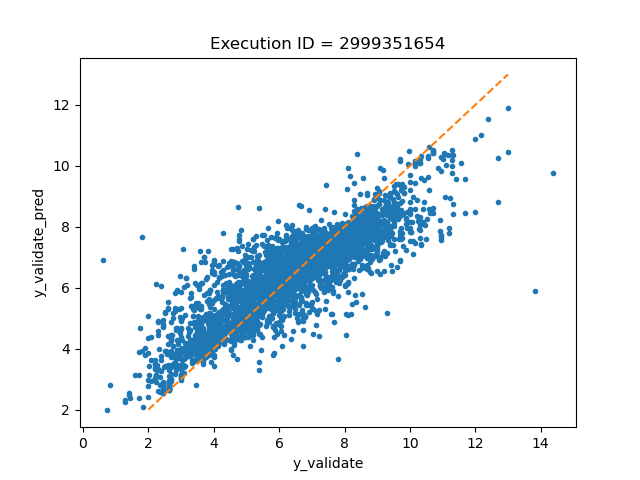
\includegraphics[scale=0.45]{images/accuracyRFRvalidate}
         \caption{Validation Accuracy}
        \label{fig:accuracyRFRvalidate}
     \end{subfigure}
     \hfill
     \begin{subfigure}[b]{0.45\textwidth}
         \centering
         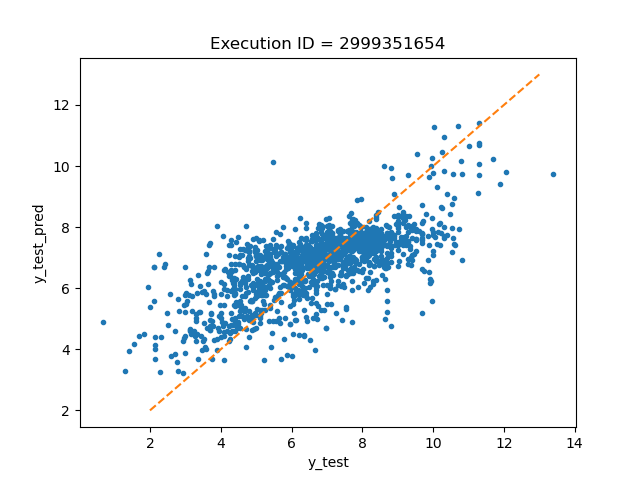
\includegraphics[scale=0.45]{images/accuracyRFRtest}
        \caption{Testing Accuracy}
        \label{fig:accuracyRFRtest}
     \end{subfigure}
     \caption{Random Forest Regressor with 176 manually selected features and hyperbolic weighting.}
     \label{fig:RFMModel}
\end{figure}

\subsubsection{Dealing with correlated features}
In Section \ref{CorrelationAnalysis} we discussed that within some of the families of features there are heavily correlated features.
One way to deal with this would be to just take one feature from a family and exclude the rest.
However, this would not be a good strategy for generalization.
This is because our trained model would be unusable by someone who could not measure one of these selected features (or if the measurements were incorrect).

For this reason,  we made use of the stochasticity of the random forest to our advantage.
During the creation of a regression tree,  the random forest model tries to get the best (feature,  value) tuple to divide the data. This is known as the split criterion.
We force it to randomly select only 20\% of the features for deciding on the split criterion.
More specifically,  we use the following values
\begin{itemize}
\item 400 Trees (n\_estimators)
\item 20\% of feature selection.  (max\_features)
\item A minimum of 2 data points for each leaf.  (min\_samples\_leaf)
\end{itemize}
These hyperparameters were determined after some empirical testing.
We increased the number of estimators as we increased the stochasticity of our ensemble.
Our model would hence be dependent on the entire family of features and not rely on a single feature heavily.


\subsubsection{Dealing with measurement resolution}

We trained our model by duplicating the data according to their weights. 
After training we got the following results - Training $R^2$ score = 0.995,  Validation $R^2$ score = 0.8298 and  Out Of Bag (OOB) score = 0.977.

We found the following issues with this strategy:
\begin{itemize}
\item The out-of-bag error (OOB score) is erroneously high here. This is because of repeated data points. Many points are both inside the selected bag and outside it.
\item Due to duplication of data points,  the trees may end up being more correlated to each other.  This will affect the generalization of our model.
\item As training this model is costly, duplicating the data points further increases the cost of training.
\end{itemize}
Hence, we conclude that duplication of the data based on their weights is a wrong strategy for this model.

When we used our weight directly in the fit function,  we could not get any noticeable improvement in our model.
We think this is because the data is already skewed towards the $\approx$2 \si{\angstrom}
data points.
This can be seen in Figure~\ref{fig:resolutiondistribution}.

\subsubsection{Feature Importance calculation}
The Random Forest regression model fitting is very expensive as compared to the simple linear regression.
For example in a machine with $4$ CPUs,  fitting a linear model on our data takes $\approx 0.51$ seconds whereas fitting the random forest model takes $\approx 25.86$ seconds.
Hence the same strategy cannot be used for feature selection as used in the linear models.
We used the following strategies to determine the importance of features in the model.

\begin{itemize}
\item \textbf{Gini Importance (or) Decrease in impurity}.  This is calculated by the model itself.
For every feature,  it calculates how much decrease in the split criterion the feature contributes in the entire ensemble (i.e in every node it's used in all the trees).
The disadvantage is that they cannot be reliable when the features have a high cardinality.  Figure~\ref{fig:GiniImportanceLabel} illustrates this importance.
\item \textbf{Permutation Importance} - This is a model agnostic method.
To calculate the importance of a feature $x$,  it takes the given data and shuffles the values of $x$.  Now the values of feature $x$ do not correspond to the correct data points,  hence there is a reduction in the prediction accuracy.
The importance of the feature is proportional to the reduction in accuracy.
The disadvantage of this method is that since each feature is checked independently,  correlated input features make the results unreliable. 
If feature $A$ and feature $B$ are correlated,  the shuffling of $A$ may not impact the model as the model can rely on $B$ for its prediction.  Figure~\ref{fig:PermutationImportanceLabel} illustrates this importance.
\end{itemize}

\begin{figure}
     \centering
     \begin{subfigure}[b]{0.45\textwidth}
         \centering
         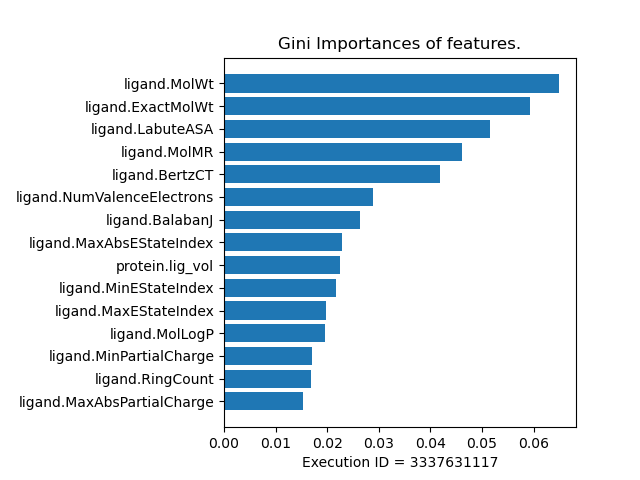
\includegraphics[scale=0.45]{images/Gini_importance}
         \caption{Gini importance}
        \label{fig:GiniImportanceLabel}
     \end{subfigure}
     \hfill
     \begin{subfigure}[b]{0.45\textwidth}
         \centering
         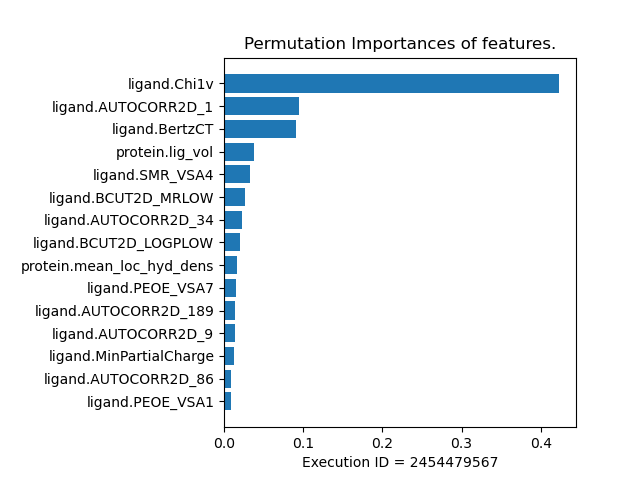
\includegraphics[scale=0.45]{images/Permutation_importance}
        \caption{Permutation importance}
        \label{fig:PermutationImportanceLabel}
     \end{subfigure}
     \caption{Feature Importance calculation of Random Forest Regressor.  (With manual feature selection)}
     \label{fig:RFMFILable}
\end{figure}

\subsubsection{Permutation Importance and genetic algorithm}
To overcome the issue with the above feature importance selection, we used a combination of permutation importance and genetic algorithm to find out the importance of the selected features.
This is because it is very expensive to refit the model and cheap enough to check the results of shuffling the model.

We used 2 different strategies to get them for our genetic algorithms -
\begin{itemize}
\item \textbf{Using specific scoring function}.  In Section ~\ref{GenerationScoringFunction},  we discussed intuition behind the scoring function used in our genetic model.
In the random forest model,  however,  this scoring function selected a lot of features ($> 400$). Hence we researched the following scoring function to reduce the number of features. 
$$
\textrm{score} = \mathbf{R}^2 * \textrm{Features Eliminated}^2
$$
We used a stronger signal for the number of eliminated features. This scoring function, however,  turned out to be too strong and none of the features were selected.
\item \textbf{Elitism}.  Elitism is a strategy used in the genetic algorithms to select the top few elements from each generation for the next generation in addition to the newly created children. This keeps the best performing subset of the population always in the current generation to improve them further by cross-over or mutation.
\end{itemize}


\subsection{Support Vector Regression}
Support vector regression is a non-linear regression method that fits a curve such that the margin of error between the model's prediction and the original value is kept within a minimum range.
Any error higher than this minimum range is penalized during the training of the model.
We trained support vector regression with the RBF kernel.

\begin{table} [h!]
\centering
\resizebox{\linewidth}{!} {
 \begin{tabular}{ | c | c | c | c | c | c | }
\hline
\textbf{No. Features} & \textbf{Feature Selection} & \textbf{Weighting} & \textbf{Training} & \textbf{Validation} &  \textbf{Testing} \\ [0.5 ex]
\hline \hline
457 & - & - & 0.310 & 0.308 & 0.356\\
457 & - & Hyperbolic & 0.325 & 0.326 & 0.371\\
\textbf{457} & \textbf{-} & \textbf{Linear}  & \textbf{0.336} &\textbf{0.334} & \textbf{0.374}\\
40 & Spearman Correlation & Linear & 0.256 & 0.286  & 0.262 \\ 
40 & Pearson Correlation & Linear & 0.199 & 0.200 & 0.199 \\ 
40 & Spearman Correlation & Hyperbolic & 0.252 & 0.266 & 0.254 \\ 
40 & Pearson Correlation & Hyperbolic & 0.169 & 0.169 & 0.169 \\ 
176 & Manual & Linear &  0.306  & 0.298  & 0.358\\ [1ex]
\hline
\end{tabular}
}
\caption{Table showing  $R^2$ Scores for SVR}
\label {table:2}
\end{table}

We did not use the duplication of data strategy for this model because the training time complexity is $O(n^2)$ where n is the number of data points.
However,  we did use data point weights during the fit function of the training.

The results are reported in Table~\ref{table:2}.
The linear weighting of the data gave the best results in SVR.
The reason testing $R^2$ score is around the same range as the training score maybe because the testing data is of better quality data as compared to the validation data.
However, this varies very highly depending on the random seed used.
What we must observe is that the approximate range in which the values are obtained is small.

As the performance of the model was not on par with other models,
we did not run the costly genetic algorithm feature selection on SVR.
Moreover,  the time it took to get the $R^2$ score (validation and testing) was very high and was not suitable to be used in a permutation-based genetic algorithm as discussed in the random forest section.
The issues of within family feature correlation as well as feature selection were hence dealt with by either using output correlation or by manual feature selection.

Figures~\ref{fig:SVRvalidate} and ~\ref{fig:SVRtest} visualize the validation and testing accuracy of the best SVR model.

\begin{figure}
     \centering
     \begin{subfigure}[b]{0.45\textwidth}
         \centering
         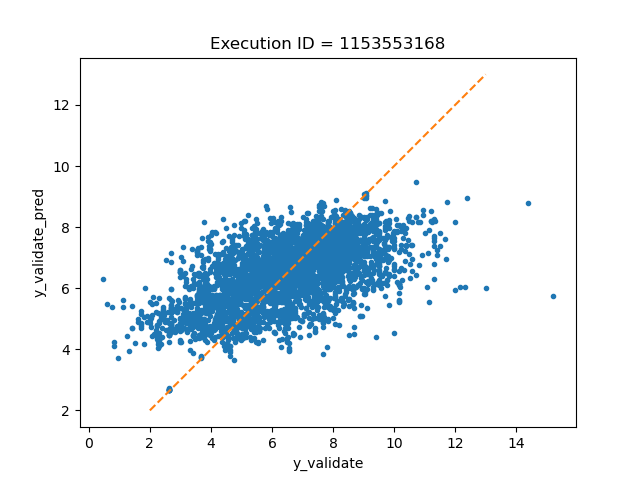
\includegraphics[scale=0.45]{images/SVRvalidate}
         \caption{Validation accuarcy}
        \label{fig:SVRvalidate}
     \end{subfigure}
     \hfill
     \begin{subfigure}[b]{0.45\textwidth}
         \centering
         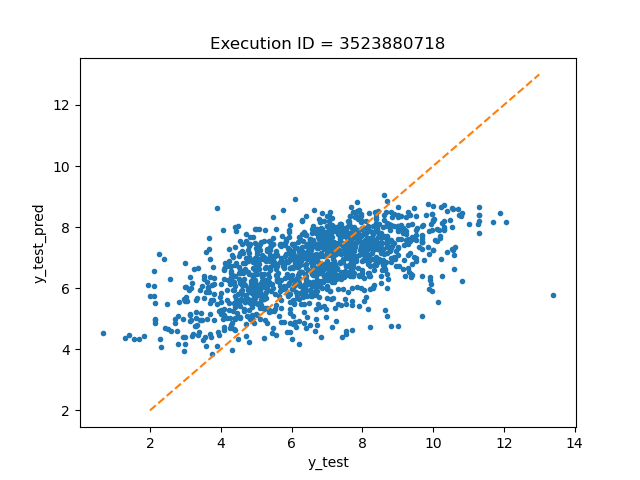
\includegraphics[scale=0.45]{images/SVRtest}
        \caption{Testing accuracy}
        \label{fig:SVRtest}
     \end{subfigure}
     \caption{SVR accuracy visualization for all features 457 and Linear weighting}
     \label{fig:SVRaccuracy}
\end{figure}


\subsection{Rotation Forests}

In Section \ref{RandomForestRegressionLabel} we analyzed different strategies to improve the performance of our model.
While fitting a tree, the random forest model tries to get a (feature, value) tuple that best divides our data.  The criterion is to reduce the entropy of the divided data.
This is done recursively till some set criteria (E.g., the leaf nodes should contain 7 data points).
However,  each (feature, value) only represents an axis-aligned hyperplane.

If there are some real-valued features in our data set,  we could reduce the complexity of our tree by using a hyperplane that is not axis aligned.
For example consider approximation of the line $y = x$.
To approximate this using an axis-aligned hyperplane,  we would require a deep tree of high complexity.
If instead, we transform our data such that the line $y = x$ transforms to $y = k$ where $k \in \mathbf{R}$,  we only require 1 (feature, value) tuple.

This can be accomplished by calculating the eigenvector of our data and transforming our feature space such that the basis vectors are the eigenvectors of the data.
Rotation forests use this concept to reduce the complexity of their trees and to get a better quality model. 
They were first proposed for classification.  We adapted the implementation for the regression case.

The training $R^2$ score was comparable to that of the random forest regressor.
However,  we did not see much improvement in the accuracy.
One of the reasons,  we hypothesize,  is that rotation forests are shown to be better than random forests only for the continuous feature values.
However,  our data set has both real-valued and discrete values,  although the discrete values are encoded as the real-values for our model.
Hence we conclude that this model is not the best model for our problem.

Table~\ref{table:4} gives an overview of the performance of Rotation forests.
The implemented model does not have an option to train weighted data.
We do not consider the models trained by using features selected by output correlation good models for similar reasons as discussed in Section \ref{RandomForestRegressionLabel}.

\begin{table} [h!]
\centering
 \begin{tabular}{ | c | c | c | c | }
\hline
\textbf{Features Selected} & \textbf{Training} & \textbf{Validation} & \textbf{Testing} \\ [0.5 ex]
\hline \hline
457 (all) & 0.967 & 0.756 & 0.543\\
457 (Hyperbolic) & NA & NA & NA\\
457 (Linear weighting) & NA & NA & NA\\
40 (Person) & 0.948 & 0.596 & 0.878\\
40 (Spearman) & 0.951 & 0.667 &0.896 \\
\textbf{176 (manual)} & \textbf{0.960} & \textbf{0.724} & \textbf{0.572} \\ [1ex]
\hline
\end{tabular}
\caption{Rotation Forest $R^2$ Score overview}
\label {table:4}
\end{table}

Figures~\ref{fig:accuracyRotationFRvalidate} and ~\ref{fig:accuracyRotationFRtest} visualize the validation and testing accuracy of the best Rotation Forest Model.

\begin{figure}
     \centering
     \begin{subfigure}[b]{0.45\textwidth}
         \centering
         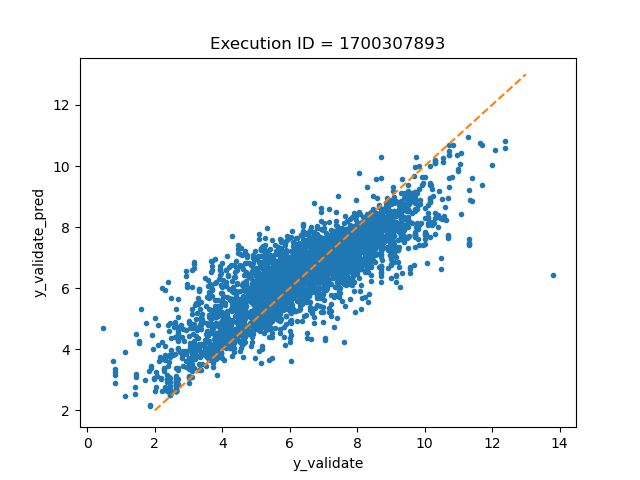
\includegraphics[scale=0.45]{images/accuracyRotationFRvalidate}
         \caption{Validation accuarcy}
        \label{fig:accuracyRotationFRvalidate}
     \end{subfigure}
     \hfill
     \begin{subfigure}[b]{0.45\textwidth}
         \centering
         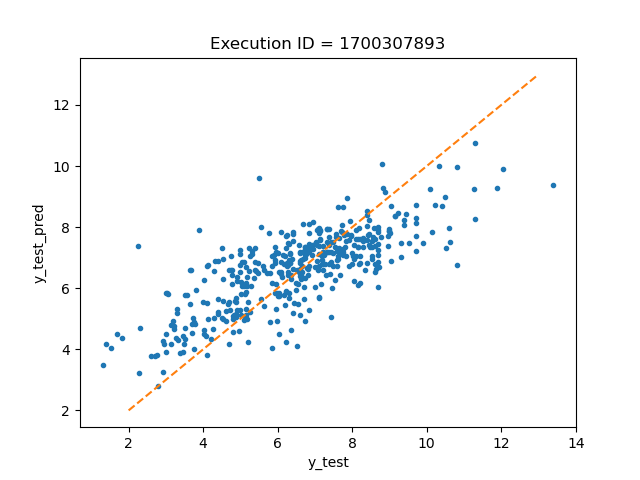
\includegraphics[scale=0.45]{images/accuracyRotationFRtest}
        \caption{Testing accuracy}
        \label{fig:accuracyRotationFRtest}
     \end{subfigure}
     \caption{Rotation Forest Accuracy visualization for manually selected features (176).  The rotation forest implementation does not support data weighting.}
     \label{fig:RotationForestAccuracy}
\end{figure}

\section{Discussion}
In this project, we tried to determine the protein-ligand binding affinity by using spatial features extracted by RDKit and D-Pocket.
We believe that 2D/3D features made our data more accessible to simple machine learning models. 
It was crucial because the complex models that directly get the 3D features from the data (E.g., 3D convolutions) require a lot of data which is expensive to accumulate.

We spent most of the time analyzing and studying the most suitable linear model (Linear Regression) and non-linear model (Random Forest Regression) for our extracted data.
Our study also included feature selection methods like genetic algorithms.
We found that our extracted protein-ligand data had the following interesting properties
\begin{itemize}
\item The data does not have a symmetric Gaussian distribution.  In other words, the ranges of values in each dimension were very different.
\item The features are both real-valued numbers as well as discrete.  The discrete values are also represented as real numbers.
\item There are feature families in the ligand descriptors that have highly correlated features.
\end{itemize}

While Linear Regression did give reasonable results,  it was not a very reliable model because it assumed that the data was linearly related to the binding affinity.
Nevertheless,  we were able to run genetic algorithms on this model to get the best $\approx$ 50 features.
We failed to do this in the case of the Random Forest Regression model.

From our study of genetic algorithms, we conclude that it was not very helpful in improving the performance of our model. However, we were able to reduce (eliminate) around 200 features for the Random Regression Model and around 400 features in the Linear Regression without hampering the performance to a large degree.

One issue with feature selection algorithms is that they make the model depend on the selected features.
This would hamper the model generalization.
A single unavailable feature or a single feature measured incorrectly would render our model useless.
This hard constraint may not be good when the data collection process is expensive and error-prone.

The Random Forest Regression model could deal with all the above specific properties of our data.
Random Forest Regression deals with both Real valued and discrete input features because the main aim of a fitting tree (in the random forest) is to reduce the entropy of the divided data.
Since all the discrete features in our data were extracted as real-valued numbers,  the trees can easily find a midpoint between the discrete values to divide the data. 
Interestingly,  the feature correlation within families can be used as an advantage to improve the robustness of the model. 
By increasing the randomness of our feature selection during the data split the model is forced to rely less on a specific feature.
Hence a wrong measurement or a corrupted feature would not hamper our model significantly.

Since the random forest model gives an $R^2$ score of $>$ 0.5 consistently,  the binding affinity predicted by the model for any new PL complex can be taken as a reference for the drug-testing decisions.
For example,  one can use the results to prioritize testing of new ligands in a wet lab experiment to save resources for the important ligands.

As with any model,  the model and approach do have limitations. 
Firstly, Random Forest Regression models cannot be explained easily.
With hundreds of trees in our random forest, the model at best can only be treated as a Black Box.
Because of its complexity,  we were not able to show why some features were very important as compared to the others (E.g., in the feature importance calculation).
Secondly, our model relies heavily on the ligand features. 
The model, hence, assumes that the binding only slightly depends on the protein features. On the contrary, the protein and ligand features are both equally responsible for the binding affinity.
Also,  hyper-parameter optimization could not be performed
in conjunction with the genetic feature selection algorithms as it was prohibitively expensive.

\section{Conclusion}
In this project, we studied methods and preprocessing techniques to predict the protein-ligand binding affinity.
In conclusion, we suggest using Random Forest Regression for this problem because of the ease of training and the generalization capability.
We believe that a random forest regression could be used as a baseline to compare any new models.

In further work,  we believe that there is scope for improving the feature selection process of our model.
Our model depends heavily on the ligand features as compared to the protein features.
We believe it is because of the data extracted by RDKit and D-Pocket.
Further investigation on new models that do not have this limitation would be helpful.
One way could be to build models with all protein features and one family of ligand features. 
The most important features in each family may can as surrogates for the whole family.
We also think more study needs to be conducted to create explainable models.
It would be both accepted by the Cheminformatics community and would be helpful to further the understanding of binding affinity.

\bibliographystyle{plain}
\bibliography{references}

\section{Appendix}
\subsection{XYZ File format}
\label{XYZFileexampleref}
The following represents the pyridine molecule in the XYZ format.
\begin{verbatim}
11

C       -0.180226841      0.360945118     -1.120304970
C       -0.180226841      1.559292118     -0.407860970
C       -0.180226841      1.503191118      0.986935030
N       -0.180226841      0.360945118      1.29018350
C       -0.180226841     -0.781300882      0.986935030
C       -0.180226841     -0.837401882     -0.407860970
H       -0.180226841      0.360945118     -2.206546970
H       -0.180226841      2.517950118     -0.917077970
H       -0.180226841      2.421289118      1.572099030
H       -0.180226841     -1.699398882      1.572099030
H       -0.180226841     -1.796059882     -0.917077970
\end{verbatim}

\subsection{SDF File format}
\label{SDFFileexampleref}
\begin{verbatim}
2uzn_ligand

Created by X-TOOL on Fri Nov 18 14:55:27 2016
 37 39  0  0  0  0  0  0  0  0999 V2000
    7.1480   60.4530    6.6830  O 0  0  0  1  0  1
    6.0470   60.1670    7.5640  S 0  0  0  1  0  4
    .......
    .......
   -2.6338   67.4589    8.1225  H 0  0  0  1  0  1
  1  2  2  0  0  2
  2  3  2  0  0  2
  .......
  .......
 23 37  1  0  0  2
M  END
> <MOLECULAR_FORMULA>
C15H13N3O4S2

> <MOLECULAR_WEIGHT>
363.3

> <NUM_HB_ATOMS>
7  

> <NUM_ROTOR>
1  

> <XLOGP2>
1.31 
\end{verbatim}

\subsection{MOL2 File Format}
\label{MOL2Fileexampleref}
\begin{verbatim}
### 
### Created by X-TOOL on Fri Sep 26 17:34:18 2014
### 

@<TRIPOS>MOLECULE
1fo2_ligand
   25    25     1     0     0
SMALL
GAST_HUCK


@<TRIPOS>ATOM
      1 C4         39.0090   40.2680   25.5130 C.3       1 DMJ         0.1280
      2 O4         39.2170   40.5810   26.8980 O.3       1 DMJ        -0.3835
     .......
     25 H14        38.0787   41.8134   21.3802 H         1 DMJ         0.2097
@<TRIPOS>BOND
     1    1    9 1  
     2    1    3 1  
    .......
    25   11   25 1  
@<TRIPOS>SUBSTRUCTURE
     1 DMJ         1
\end{verbatim}

\subsection{Correlation Heat Maps}
\label{CorrHeatMapsAppendix}
This section shows the correlation heat maps of the most interesting feature families in the our dataset.
\begin{figure}
     \centering
     \begin{subfigure}[b]{0.45\textwidth}
         \centering
    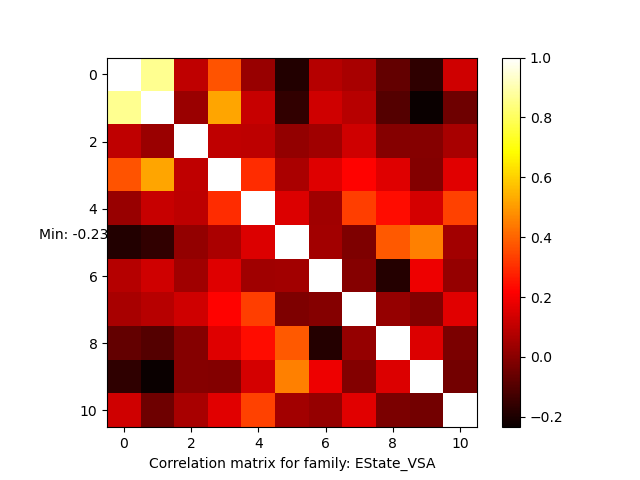
\includegraphics[scale=0.5]{images/correlationEStateVSA}
    \caption{Family EState\_VSA}
    \label{fig:correlationEStateVSA}
     \end{subfigure}
     \hfill
     \begin{subfigure}[b]{0.45\textwidth}
         \centering
        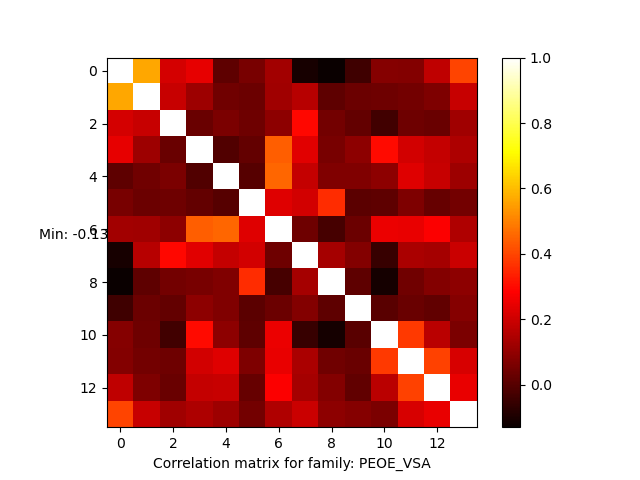
\includegraphics[scale=0.5]{images/correlationPEOEVSA}
        \caption{Family PEOE\_VSA}
        \label{fig:correlationPEOEVSA}
     \end{subfigure}
          \hfill
     \begin{subfigure}[b]{0.45\textwidth}
         \centering
        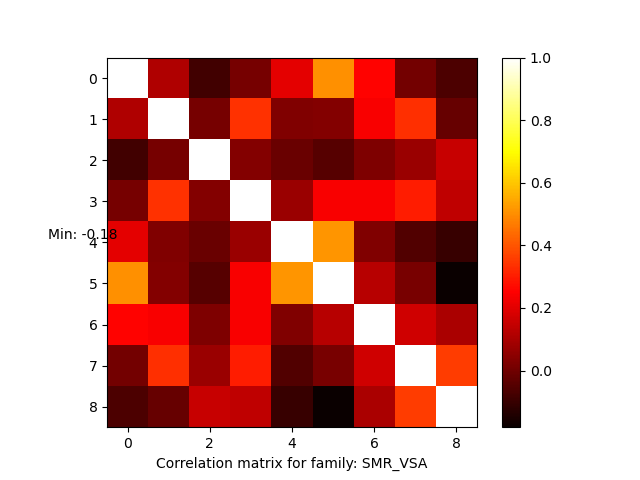
\includegraphics[scale=0.5]{images/correlationSMRVSA}
        \caption{Family SMR\_VSA}
        \label{fig:correlationSMRVSA}
     \end{subfigure}
               \hfill
     \begin{subfigure}[b]{0.45\textwidth}
         \centering
        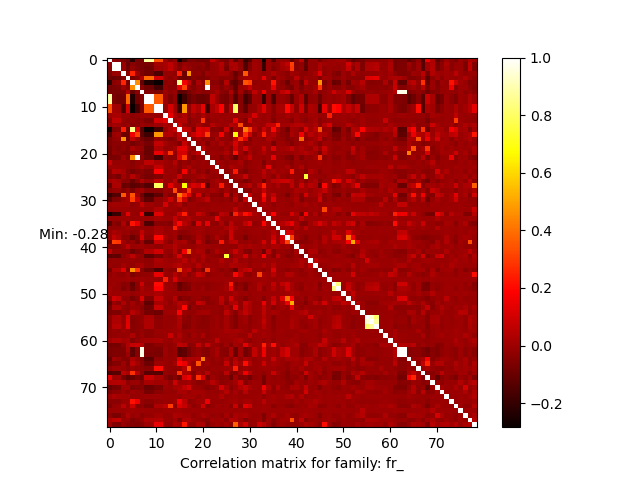
\includegraphics[scale=0.5]{images/correlationfr}
        \caption{Family fr\_}
        \label{fig:correlationfr}
     \end{subfigure}
      \hfill
     \begin{subfigure}[b]{0.45\textwidth}
         \centering
        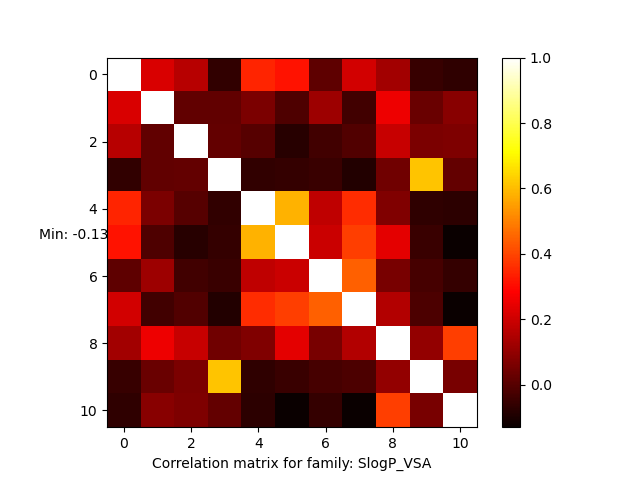
\includegraphics[scale=0.5]{images/correlationSlogPVSA}
        \caption{Family SlogP\_VSA}
        \label{fig:correlationSlogPVSA}
     \end{subfigure}
             \hfill
     \begin{subfigure}[b]{0.45\textwidth}
         \centering
        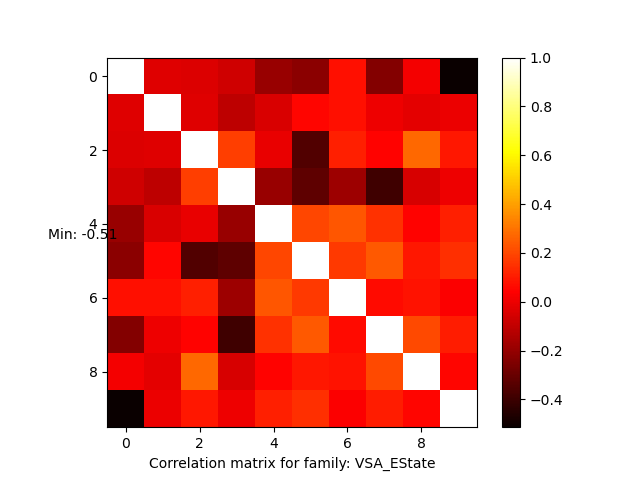
\includegraphics[scale=0.5]{images/correlationVSAEState}
        \caption{Family VSA\_EState}
        \label{fig:correlationVSAEState}
     \end{subfigure}     
     \caption{Correlation Heat Maps}
     \label{fig:CorrHeatMapFig}
\end{figure}

\end{document}

